\begin{song}{title=\predtitle\centering Vlaštovky \\\large Traband  \vspace*{-0.3cm}}  %% sem se napíše jméno songu a autor
\begin{centerjustified}

\sloka 
	^{Dmi\z}Každé jaro ^{Ami\z}z~velké dáli ^{B\z }vlaštovky k nám ^{F\z }přilétaly,

	^{Dmi\z }někdy až ^{C\z }dovnitř do ^{\z Ami}stavení.

	^{Dmi}Pod střechou se ^{Ami\z }uhnízdily a ^{B\z }lidé, kteří uvnitř ^{F\z }žili,
	
	^{Dmi\z }rozuměli ^{C\z }jejich ^{\z Ami}švitoření.


\sloka 
	O dalekých krajích, hlubokých mořích, divokých řekách,

	o vysokých horách, které je nutné přelétnout,

	o nebeských stezkách, zářících hvězdách, o cestách domů,

	o korunách stromů, kde je možné odpočinout.


\sloka 
	Jsme z míst, která jsme zabydlili,

	z hnízd, která jsme opustili,

	z cest, které končí na břehu.

	Jsme z lidí i všech bytostí,

	jsme z krve, z masa, z kostí,

	jsme ze vzpomínek, snů a příběhů.


\sloka 
	Jsme jako ti ptáci, z papíru draci, létáme v mracích

	a pak se vracíme zpátky tam, kde připoutaní jsme.

	Jsme lidské bytosti z masa a kostí, jsme jenom hosti

	na tomhle světě -- přicházíme, odcházíme.


\sloka 
	A chceme mít jisto, že někde je místo, že někde je hnízdo,

	odkud jsme přišli a kam zas potom půjdeme spát,

	že někde je domov, že někde je hnízdo, útulno čisto,

	že někde je někdo, kdo čeká na nás, na návrat.


\sloka 
	Tam v dalekých krajích, v hlubokých mořích, v divokých řekách,

	ve vysokých horách, které je nutné přelétnout.

	Tam v nebeských stezkách, v zářících hvězdách, na cestách domů,

	v korunách stromů, kde je možné odpočinout.

\end{centerjustified}

\centering
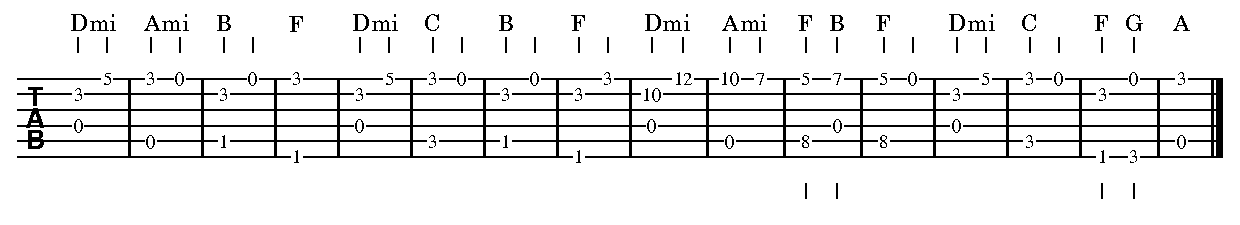
\includegraphics[scale=\defaulttabscale]{../taby/vlastovky.pdf}

\setcounter{Slokočet}{0}
\end{song}
